\documentclass[11pt,letter]{article}
\usepackage{amsmath, amsthm, amssymb}
\usepackage{eucal, mathrsfs, yfonts}
\usepackage{amsfonts}
\usepackage{amssymb}
\usepackage{amsmath}
\usepackage{amsthm}
\usepackage{verbatim}
\usepackage{fancyhdr}
\usepackage{geometry}
\usepackage{setspace}
\usepackage{Tabbing}
\usepackage{lastpage}
\usepackage{extramarks}
\usepackage{chngpage}
\usepackage{soul,color}
\usepackage{graphicx,float,wrapfig}
\usepackage[urlcolor=blue]{hyperref}
\hypersetup{colorlinks=true}

\graphicspath{{./Pictures/}}

%code preamble
\usepackage{color}
\usepackage{xcolor}
\usepackage{listings}

\usepackage{caption}
\DeclareCaptionFont{white}{\color{white}}
\DeclareCaptionFormat{listing}{\colorbox{gray}{\parbox{\textwidth}{#1#2#3}}}
\captionsetup[lstlisting]{format=listing,labelfont=white,textfont=white}

\lstset{language=C++,
               basicstyle=\ttfamily\small,
               keywordstyle=\color{blue}\ttfamily,
               otherkeywords={WIDTH},
               keywords=[2]{__shared__},
               keywordstyle=[2]\color{orange}\ttfamily,
               stringstyle=\color{green}\ttfamily,
               commentstyle=\color{red}\ttfamily,
               breaklines=true,
}
%end code preamble

\topmargin=-0.45in      %
\evensidemargin=0in     %
\oddsidemargin=0in      %
\textwidth=6.5in        %
\textheight=9.0in       %
\headsep=0.25in         %


\newcommand{\HRule}{\rule{\linewidth}{0.5mm}}

\pagestyle{fancy}

%-------------------------------------------------------------------------
%TITLE AND HEADERS
%-------------------------------------------------------------------------

\lhead{Asssignment 2}
\chead{UCID: 22365174}
\rhead{Arturo Pacifico Griffini}

\title{Assignment 1 }
\author{Arturo Pacifico Griffini\\
  UCID: 22365174}
\date{}

\begin{document}
%\maketitle
%\input{./title.tex}

\pagebreak

%-------------------------------------------------------------------------
%PROBLEMS
%-------------------------------------------------------------------------


\section{Vectorization}
\subsection{Code}
\begin{lstlisting}[label=some-code,caption=vector\_blur.cpp]
#include "my_blurs.h"

using namespace std;

void vector_blur(float* out, int n, float* frame, int* radii){
  for(int r=0; r<n; r++)
    for(int c=0; c<n; c++){
      int rd = radii[r*n+c];
      int num = 0;
      float avg = 0;
      __m128 avg4 = _mm_set1_ps(0);
      for(int r2=max(0,r-rd); r2<=min(n-1, r+rd); r2++) {
	for(int c2=max(0, c-rd); c2<=min(n-1, c+rd);){
	  if (c2 + 4 <= min(n-1, c+rd)) {
            __m128 vals = _mm_loadu_ps(frame + r2*n + c2);
            avg4 = _mm_add_ps(avg4, vals);
	    num += 4;
	    c2 += 4;
          } else {
            avg += frame[r2*n+c2];
	    num += 1;
            c2 += 1;
          }
	}
      }
      float avg_a[4];
      _mm_storeu_ps(avg_a, avg4);
      for (int i = 0; i < 4; i++)
	avg += avg_a[i];
      out[r*n+c] = avg/num;
    }
}
\end{lstlisting}

\subsection{How Much Faster}
The vectorised code ran $1.54$ times faster than the naive blur. Ideally, we should get up to $4$ times faster. However, the reduced performance it is probably due to two factors. Firstly, the ratio of edge cases (where we cannot properly use SIMD instructions) to good cases (where we can use the SIMD efficiently) is relatively high, and this is true for small blurring radiuses and resolution. Secondly, we are adding some floating point adds to accumulate the values of the vectors. 

\subsection{Kernel Organisation}
Let $p_{r, c}$ be  a pixel in position $(r, c)$  in the blurring frame, and define the SIMD vector $\mathbf{V} = \left< v_0, v_1, v_2, v_4\right>$ with $$v_t = \sum_{i, j \equiv t \bmod 4} p_{i, j}$$
So, for each row of the pictures we are accumulating all the pixels with column value $ \equiv t \bmod 4$, in the frame, to $v_t$. Then, once we reach the end of the pixels in the frame we accumulate the four values to the sum used for the blurring. 
\subsection{Aligned/Unaligned Loads}
Intel states that "If alignment cannot be guaranteed, some part of the performance gain achieved by processing multiple data elements in parallel will be lost because either the compiler or assembly programmer must use unaligned move instructions," which for most architectures are slower than aligned move instruction. In this implementation, aligned instructions were not utilised due to simplicity. One approach would be to use the vectorization on aligned memory blocks of 4 floats within the blurring frame and then deal with the edge cases using the unvectorized approach to the algorithm. Using Intel's reference on SIMD, this implementation should have a speedup of something below 2x on Core i7 CPU.

\section{Parallelization}
\subsection{Code}
\begin{lstlisting}[label=some-code,caption=parallel\_blur.cpp]
#include "my_blurs.h"

using namespace std;

void parallel_blur(float* out, int n, float* frame, int* radii){
#pragma omp parallel for schedule(dynamic)
  for(int r=0; r<n; r++)
    for(int c=0; c<n; c++){
      int rd = radii[r*n+c];
      int num = 0;
      float avg = 0;
      for(int r2=max(0,r-rd); r2<=min(n-1, r+rd); r2++)

	for(int c2=max(0, c-rd); c2<=min(n-1, c+rd); c2++){
          avg += frame[r2*n+c2];
          num++;
	}
      out[r*n+c] = avg/num;
    }
}

\end{lstlisting}
\pagebreak

\subsection{Scaling Plot}
\begin{figure}[h]
\centering
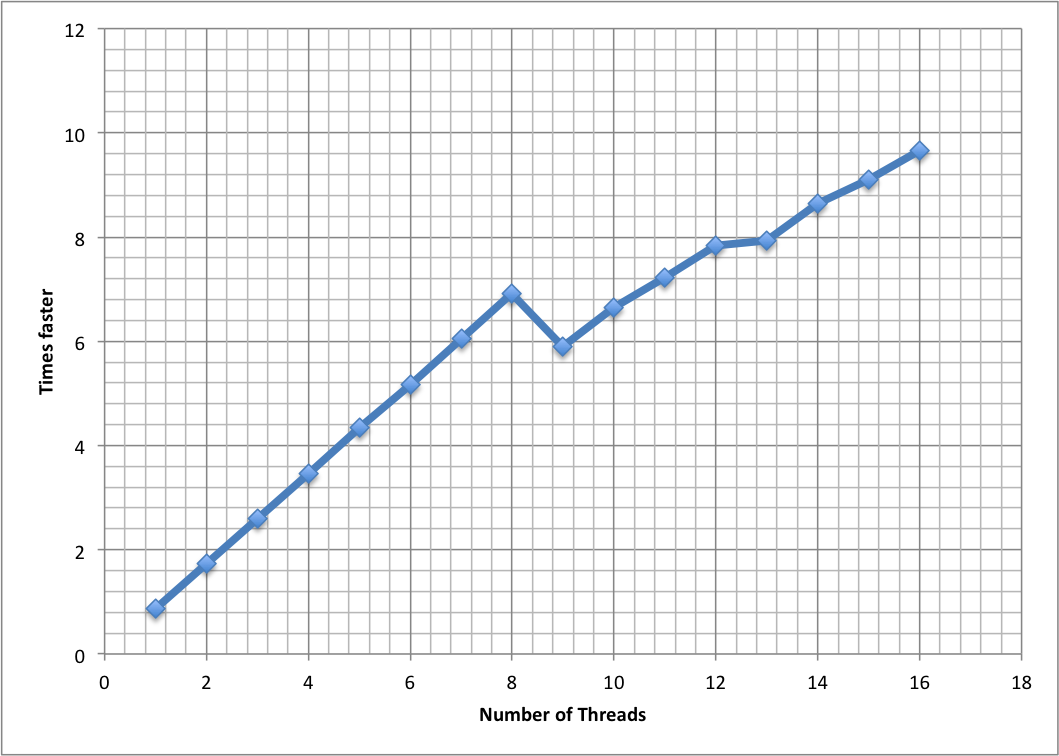
\includegraphics[width=0.8\textwidth]{graph.png}
\caption{Scaling Plot}
\label{fig:awesome_image}
\end{figure}
\subsection{Kernel Organisation}
We simply assign every row of the picture frame to a different thread using parallel for flag on the outer loop of the algorithm. 

\subsection{Load Balancing}
Load balancing was approached using the $schedule$ flag with $dynamic$ option on parallel for flag. Threads that are closer to the top and bottom frames will do less work than threads in the centre of the picture frames. The dynamic option will balance the load at run time.


\section{Fastest Implementation}
\subsection{Code}
\begin{lstlisting}[label=some-code,caption=fastest\_blur.cpp]
#include "my_blurs.h"

using namespace std;

void fastest_blur(float* out, int n, float* frame, int* radii){
#pragma omp parallel for schedule(dynamic)
  for(int r=0; r<n; r++)
    for(int c=0; c<n; c++){
      int rd = radii[r*n+c];
      int num = (max(0,r-rd) - min(n-1, r+rd) - 1) * (max(0, c-rd) - min(n-1, c+rd) - 1);
      float avg = 0;
      __m128 avg4 = _mm_set1_ps(0);
      for(int r2=max(0,r-rd); r2<=min(n-1, r+rd); r2++) {
	for(int c2=max(0, c-rd); c2<=min(n-1, c+rd);){
          if (c2 + 4 <= min(n-1, c+rd)) {
	    __m128 vals = _mm_loadu_ps(frame + r2*n + c2);
            avg4 = _mm_add_ps(avg4, vals);
            c2 += 4;
          } else {
            avg += frame[r2*n+c2];
            c2 += 1;
          }
	}
      }
      float avg_a[4];
      _mm_storeu_ps(avg_a, avg4);
      for (int i = 0; i < 4; i++)
	avg += avg_a[i];
      out[r*n+c] = avg/num;
    }
}
\end{lstlisting}

\subsection{How Much Faster}
The fastest implementation is $11.6$ times faster than the naive blur. 
\subsection{Configuration}
We simply assign every row of the picture frame to a different thread using parallel for flag on the outer loop of the vectorised algorithm.

%\begin{lstlisting}[label=some-code,caption=Random Permutation with 1 cycle]
%
%\end{lstlisting}


%\begin{figure}[h]
%\centering
%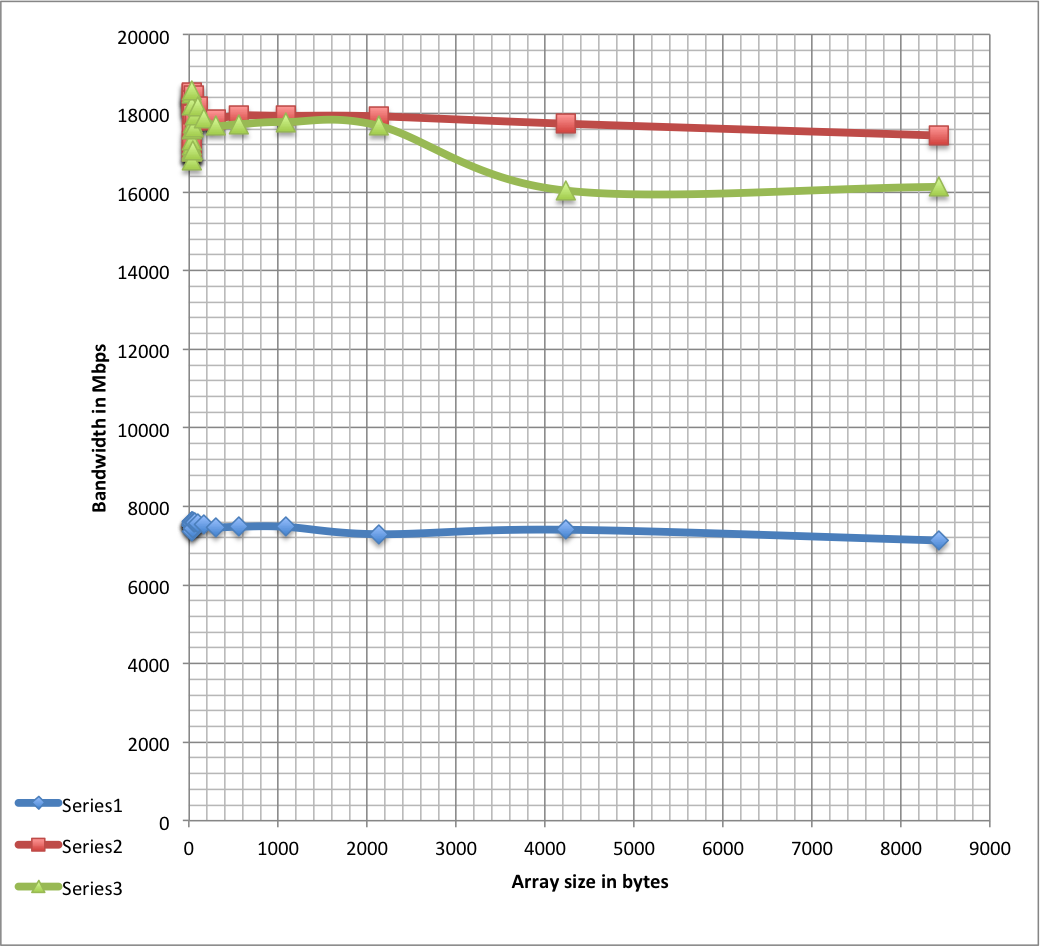
\includegraphics[width=0.8\textwidth]{graph_mem.png}
%\caption{series 1: inefficient routine; series 2: simd\_memcpy; series 3: simd\_memcpy\_cache}
%\label{fig:awesome_image}
%\end{figure}



\end{document}








% \begin{lstlisting}[label=some-code,caption=Some Code]
% public void here() {
% goes().the().code()
% }
% \end{lstlisting}








